\documentclass[12pt]{article}
\usepackage{graphicx}
\begin{document}

\title{P2 Architecture}
\author{The P2 Team}
\maketitle

\section{Introduction}

This design document outlines the major components of the next generation P2
Architecture. The main components of the new architecture are illustrated in 
Figure~\ref{fig:arch}. Much of the design revolves around the processing of 
\emph{task} objects. There are two types of tasks in this system design, 
\emph{EVENT} and \emph{ACTION}. These two tasks are motivated by the 
OverLog Semantics design document. 

An EVENT task represents the object that Rule strands operate on. As stated in the OverLog document, the schedular schedules a single EVENT during each 
round~\footnote{A round is defined as the processing of an EVENT task and all of its
resulting ACTION tasks.}. Each event could trigger one or more rule strands. The 
output of a rule strand is an ACTION task. All ACTION tasts are feed into the P2 
Kernel Action Handler, which are upcalled to the appropriate P2 micro-kernel. The 
P2 Kernel also handles any events that emanate from the P2 micro-kernels in its
Event Handler. The remainder of this document details the operational semantics 
of each system component.

\begin{figure*}
   \centering
   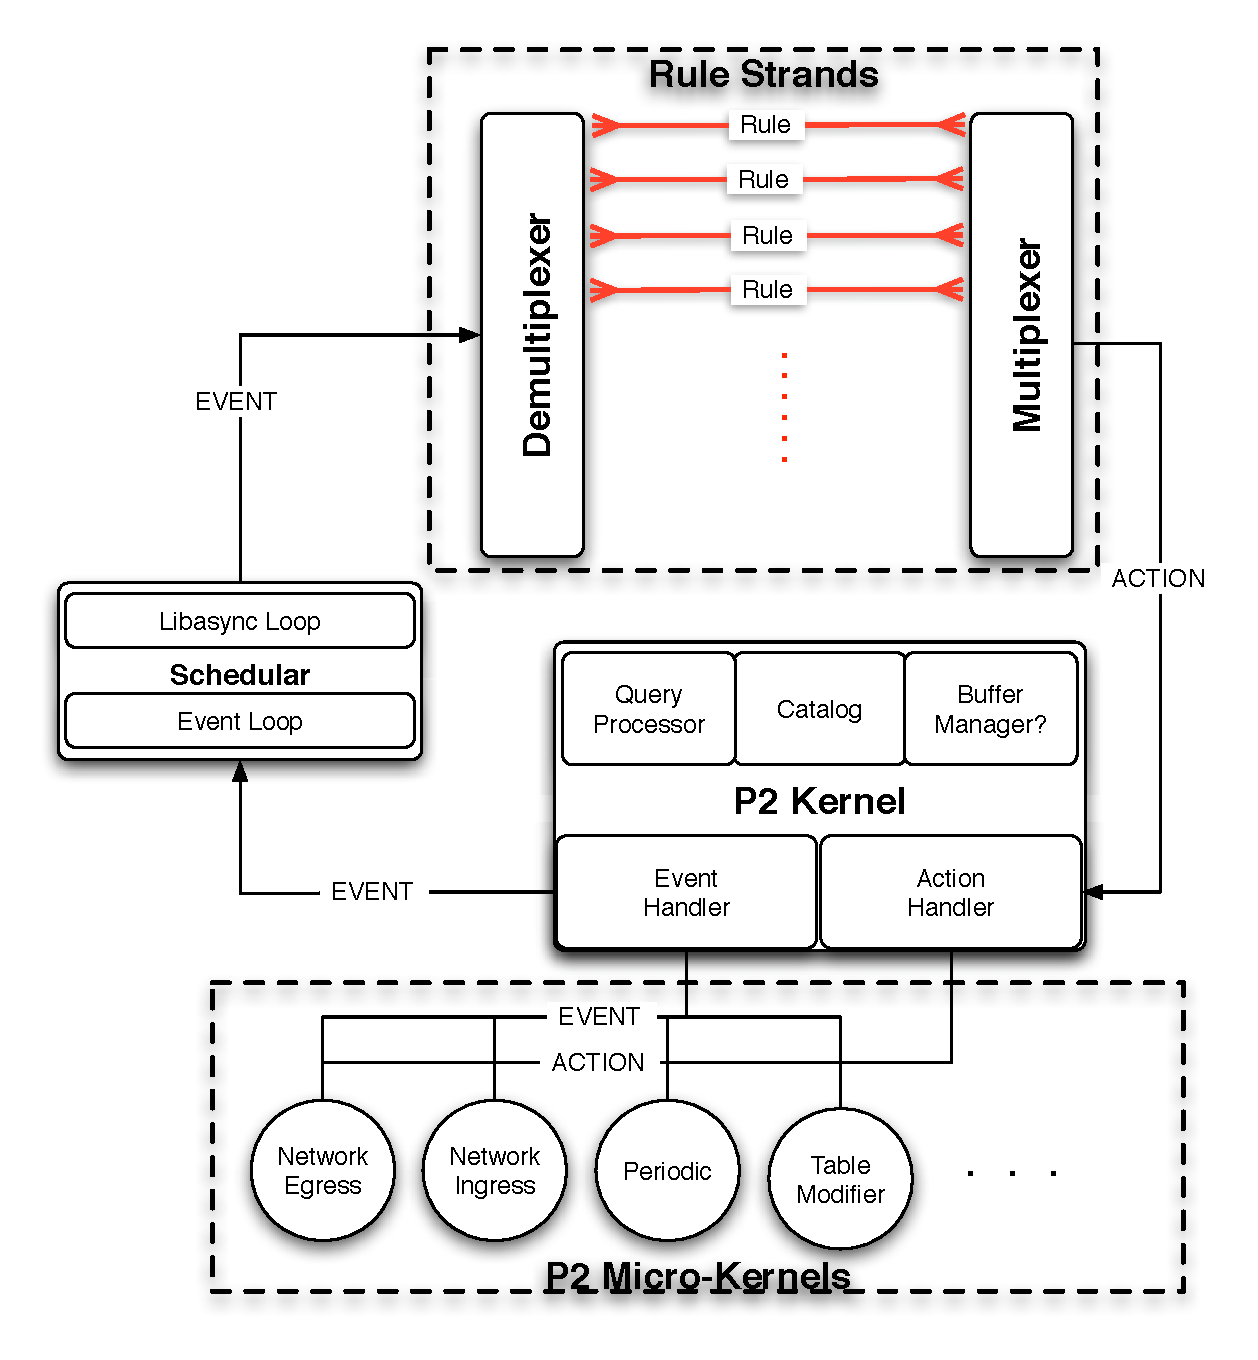
\includegraphics[width=6in]{p2-arch.eps} 
   \caption{Abstract view of the P2 Architecture.}
   \label{fig:arch}
\end{figure*}

\newpage

\section{P2 Kernel}
At the heart of the P2 architecture lies the P2 Kernel. The primary purpose of this
component is to house system components that do not (only) operate on \emph{tasks}. 
During system bootstrap, this component will initialize the subcomponents shown
in the figure. 

The Query Processor contains the OverLog compiler and the logic that
manages (e.g., allocates and deallocates) rule strands.  The Catalog holds definitions
used by the Query Processor to semantically check action rules. There is a clear need
for some kind of Buffer Manager if we wish to support disk based tables and query plans
(e.g., joins). However, this component is not on the critical path and is therefore at a 
very low priority on the development front. 

The P2 Kernel contains both Event and Action Handlers. The Event Handler is
the interface used by the P2 Micro-Kernels when an EVENT is generated. On recept
of an EVENT, the Event Handler performs some minimal processing (e.g., logging, 
statistics, etc.) before potentially passing it along to the Schedular. The Action Handler
processes the ACTION tasks the are produced from the Rule Strands. There will also
likely be some syscall/callback interface to the Action Handler that the Schedular can 
use to determine if all actions have been executed.

\section{Micro-kernels}

The P2 Micro-kernels process ACTION tasks and produce EVENT tasks. A few example micro-kernels are shown in the figure. A micro-kernel can be allocated at either 
bootstrap time or during the compilation of some OverLog rule. For instance, both 
Network Egress and Ingress would be generated by the system bootstrap routine. While
Periodic and Table Modifier components would be created based on an OverLog rule.


\section{Schedular}

The Schedular schedules EVENT tasks and manages the Libasync Loop used by
system dataflows to schedule callbacks. The scheduling algorithm for the initial version
will likely be simple FIFO. A single EVENT will be scheduled once all ACTION tasks
of the EVENT task prior to it have been executed. The Schedular will use its knowledge 
of the Libasync Loop and the Action Handler interface to determine that all ACTION 
tasks have reached a quiescent state.

\section{Rule Strands}
A set of rule strands, determined by the Query Processor, are maintained by an
EVENT Demultiplexer and ACTION Multiplexer. This Demux and Mux will need to
be specialized and allow for runtime expansion/retraction of rules. 

A rule strand is the dataflow representation of some \emph{action} rule, as defined in 
the OverLog semantic document. The input to an action rule is an EVENT task and
the output is an ACTION task. The Demux will copy an EVENT task to all rule inputs
that understand the EVENT. All ACTION tasks are feed into the P2 Kernel Action Handler
where they will be directed to the appropriate micro-kernel.

\end{document}
 